\chapter{How to cool very hot surfaces}
\section{Introduction}
\begin{table}[H]
    \centering
    \begin{tabular}{@{}lll@{}}
        \toprule
        \textbf{Context} & \textbf{Material development} & \textbf{Design}\\
        \midrule
        Gas turbine engines & Material development & TBC\\
        & manufacturing techniques & air cooling\\
        Re-entry spacecraft & Surface properties & Angle of attack\\
        & ablation & changing geometry\\
        Silicon processors & None really - still with silicon & Clamp on cooling system\\
        & with an adhesive metal plate\\
        \bottomrule
    \end{tabular}
    \caption{Introduction.}
\end{table}
\section{Jet engines}
Purpose is to convert chemical energy into linear momentum (IC engine - chemical energy into pressure).
\begin{figure}[H]
    \centering
    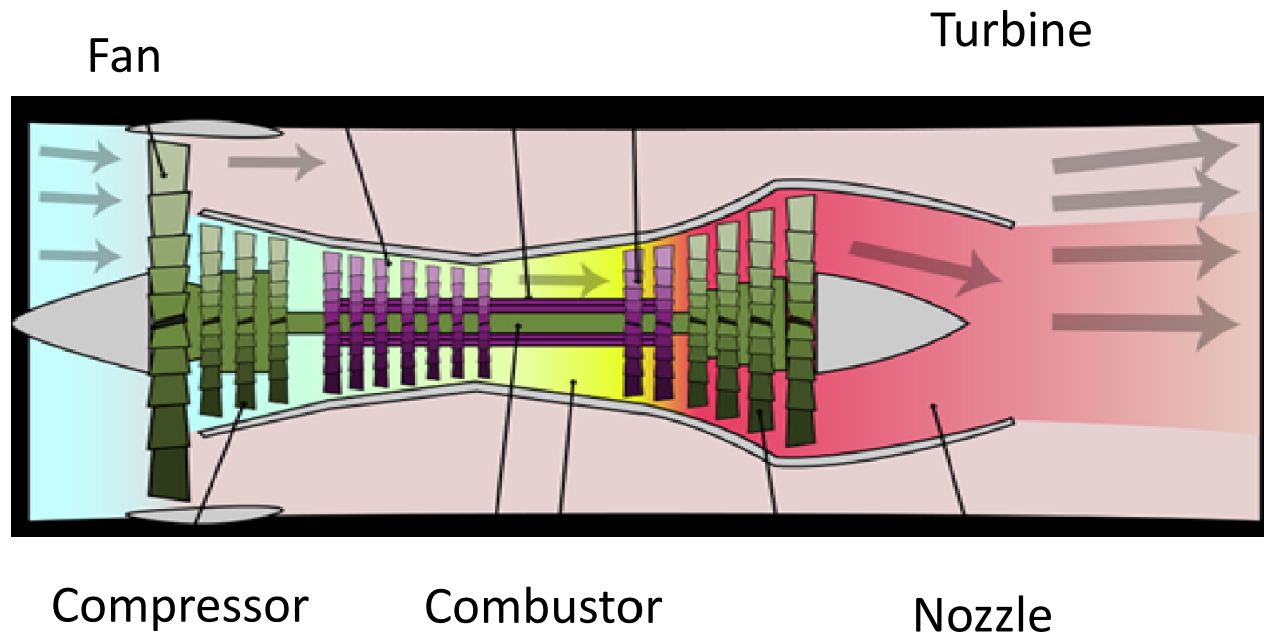
\includegraphics[width = 0.8\textwidth]{img/figure19.png}
    \caption{Jet engine.}
\end{figure}
\subsection{Brayton (or Joule) cycle}
\begin{figure}[H]
    \centering
    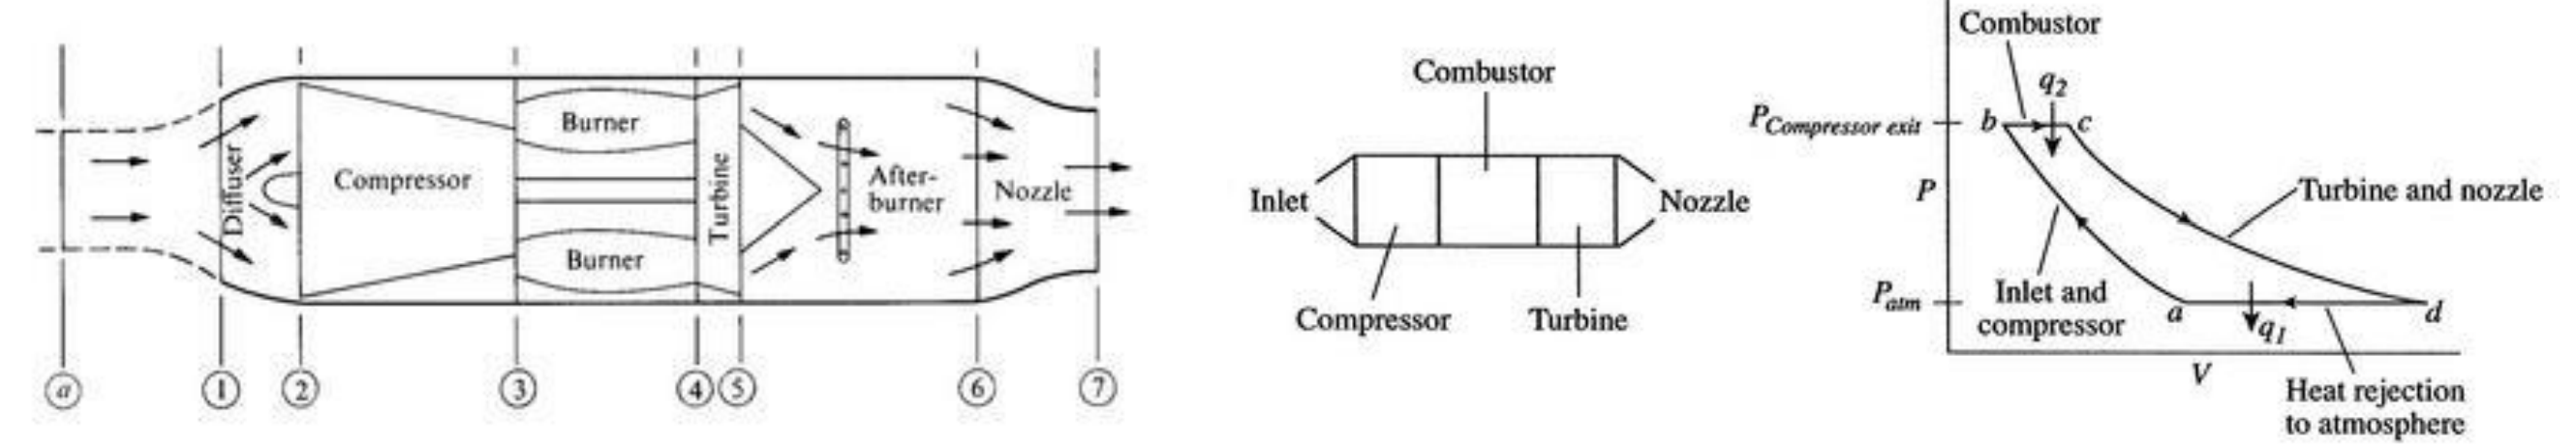
\includegraphics[width = \textwidth]{img/figure20.png}
    \caption{Brayton (or Joule) cycle.}
\end{figure}
\begin{itemize}
    \item a-b: adiabatic, quasi-static (or reversible) compression in the inlet and compressor
    \item b-c: constant pressure fuel combustion (idealised as constant pressure heat addition)
    \item c-d: adiabatic, quasi-static (or reversible) expansion in the turbine and exhaust nozzle, with which we take some work out of the air and use it to drive the compressor and take the remaining work out and use it to accelerate fluid for jet propulsion, or to turn a generator for electrical power generation
    \item d-a: cool the air at constant pressure back to its initial condition
\end{itemize}
\begin{itemize}
    \item \textbf{Fan} - the large spinning fan sucks in large quantities of air. It then speeds this air up and splits it into two parts. One part continues through the ``core'' or centre of the engine, where it is acted upon by the other engine components. The second part ``bypasses'' the core of the engine. It goes through a duct that surrounds the core to the back of the engine where it produces much of the force that propels the airplane forward. The cooler air helps to quiet the engine as well as adding thrust to the engine.
    \item \textbf{Compressor} - the compressor is the first component in the engine core. The compressor squeezes the air that enters it into progressively smaller areas, resulting in an increase in the air pressure. This results in an increase in the energy potential of the air. The squashed air is forced into the combustion chamber. 
    \item \textbf{Combustor} - in the combustor the air is mixed with fuel and then ignited. THis provides a high temperature, high-energy airflow. The fuel burns with the oxygen in the comrpessed air, producing hot expanding gases. The inside of the combustor is often made of ceramic materials to provide a heat-resistant chamber. The temperature can reach \SI{2700}{\degree C}
    \item \textbf{Turbine} - the high-energy airflow coming out of the combustor goes into the turbine, causing the turbine blades to rotate. The turbines are linked by a shaft to turn the blades in the compressor and spin the intake fan at the front. This rotation takes some energy from the high-energy flow that is used to drive the fan and the compressor. The gases produced in the combustion chamber move through the turbine and spin its blades. The turbines of the jet spin around thousands of times. They are on fixed shafts which have several sets of ball-bearings in between them.
    \item \textbf{Nozzle} - the nozzle produces the thrust for the plane. The energy depleted airflow that passed the turbine in addition to the colder air that bypassed the engine core, produces a force when exiting the nozzle that acts to propel the engine, and therefore the airplane, forward. The combination of the hot air and cold air are expelled and produce an exhaust, which causes a forward thrust. The nozzle may be preceded by a mixer, which combine the high temperature air coming from the engine core with the lower temperature air that was bypassed in the fan. The mixer helps to make the enginer quieter. 
\end{itemize}
\subsection{Typical values}
\begin{figure}[H]
    \centering
    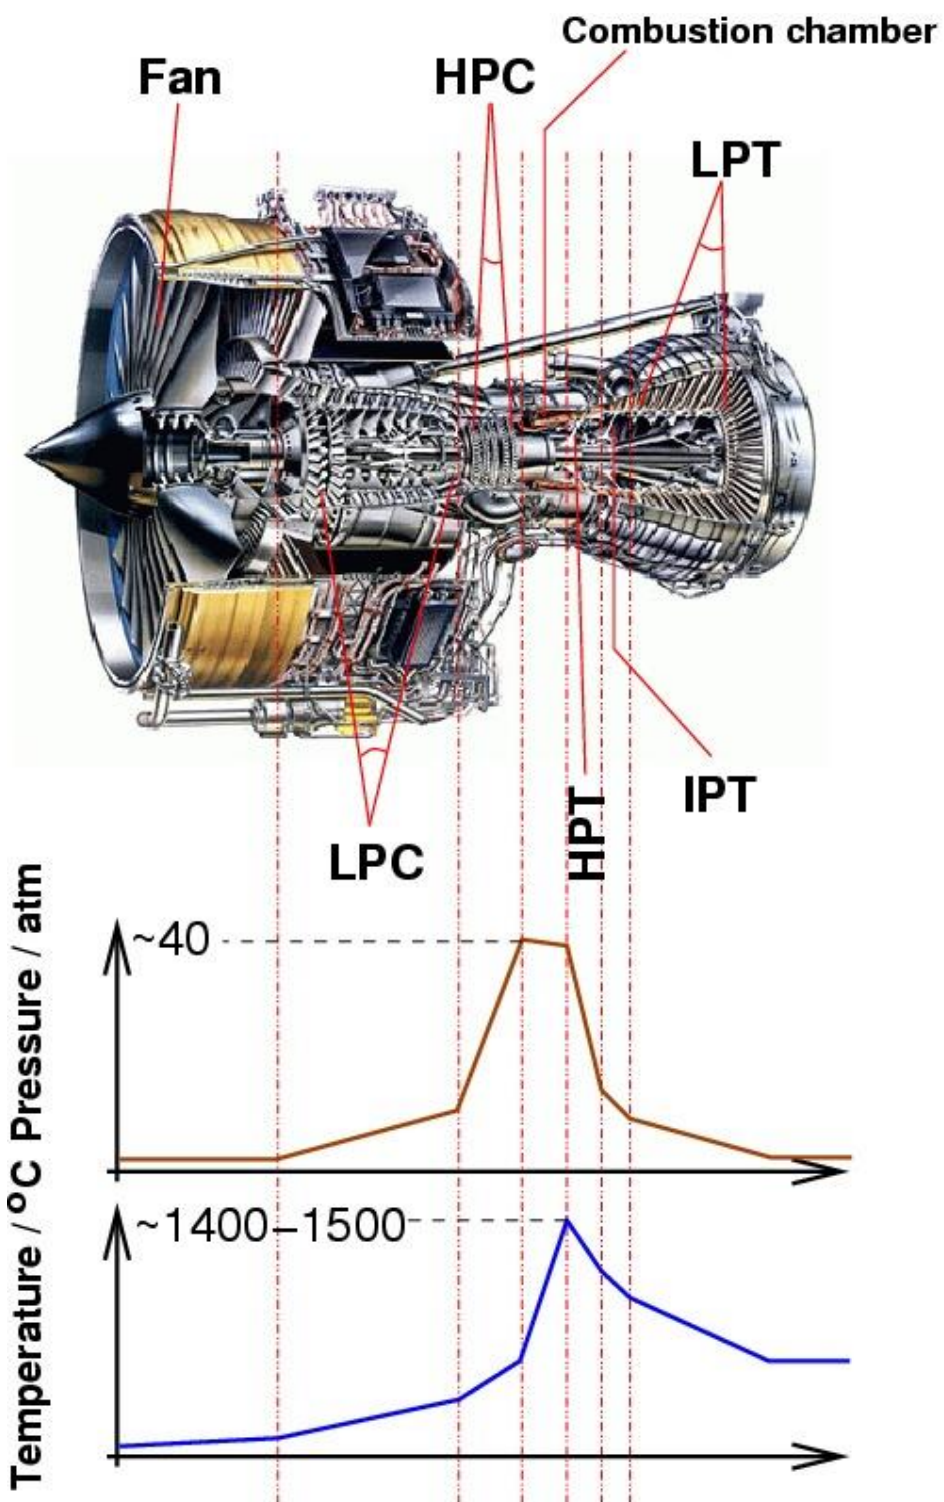
\includegraphics[width =0.5\textwidth]{img/figure21.png}
    \caption{Typical temperature values for different stages of cycle in bypass gas-turbine engine.}
\end{figure}
\begin{table}[H]
    \centering
    \begin{tabular}{@{}ll@{}}
        \toprule
        \textbf{Metal} & \textbf{Melting point}\\
        \midrule
        Titanium & \SI{1668}{\degree C}\\
        Nickel & \SI{1455}{\degree C}\\
        Steel & \SI{1370}{\degree C}\\
        \bottomrule
    \end{tabular}
    \caption{Table to show melting points of various metals used in bypass gas-turbine engines.}
\end{table}
Combustion at about 1800-\SI{1900}{\degree C}. Large centrifugal acceleration \SI{25000}{rpm} for large engines \SI{500000}{rpm} for micro gas turbine. Higher temperature makes the thermodynamic efficiency greater (about 60\%). Combustion temperature is above melting point of metals. 
\begin{table}[H]
    \centering
    \begin{tabular}{@{}ll@{}}
        \toprule
        \textbf{Fuel} & \textbf{Combustion temperature}\\
        \midrule
        Methane (in air) & \SI{1950}{\degree C}\\
        Hydrogen (in air) & \SI{2110}{\degree C}\\
        Propane (in oxygen) & \SI{2880}{\degree C}\\
        \bottomrule
    \end{tabular}
    \caption{Table to show combustion temperatures of various fuels.}
\end{table}
\subsubsection{Meeting the needs}
\begin{enumerate}
    \item Choice of material
    \item Manufacturing technique
    \item Design
\end{enumerate}
\begin{figure}[H]
    \centering
    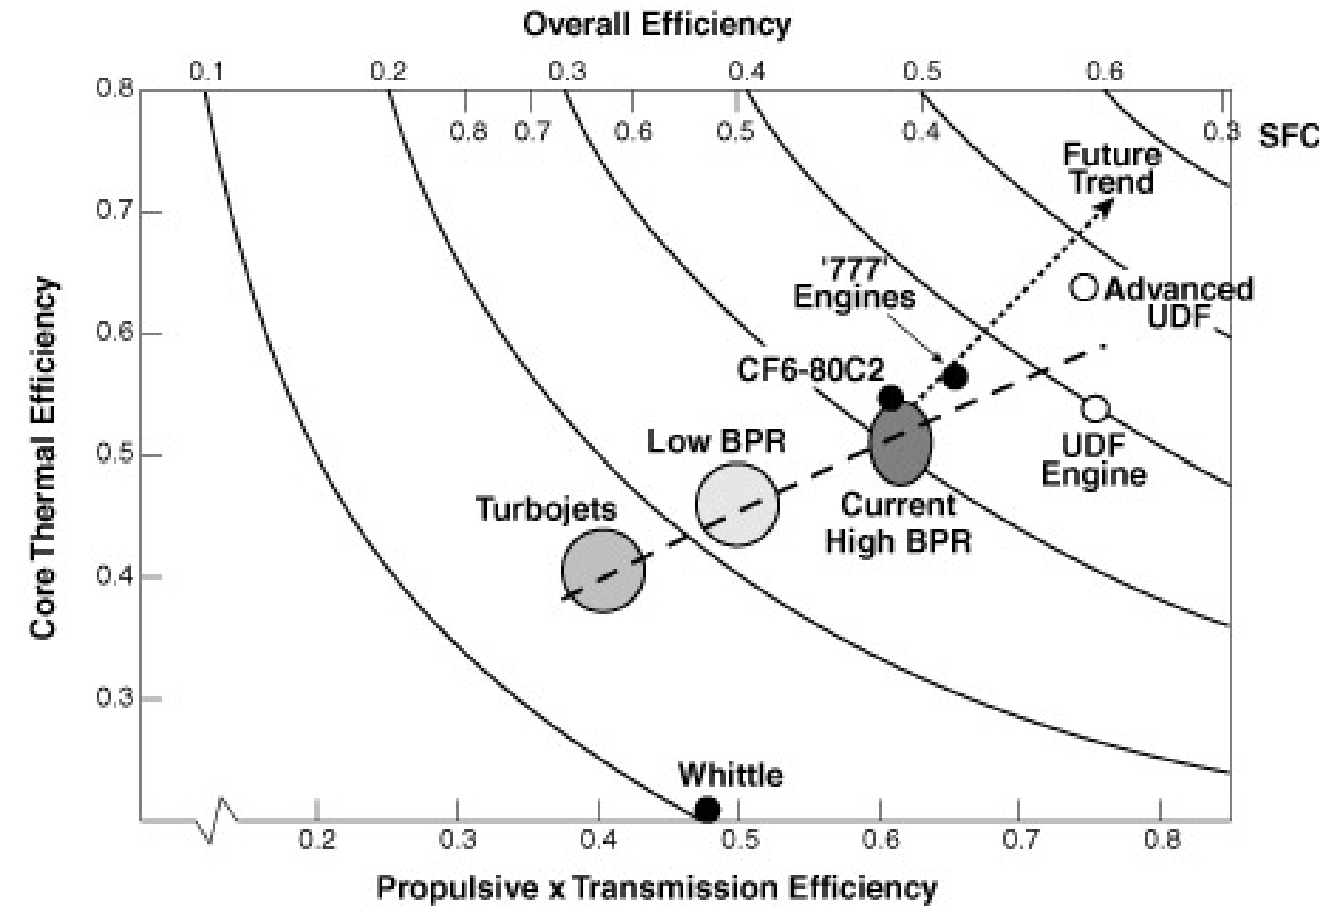
\includegraphics[width =0.8\textwidth]{img/figure22.png}
    \caption{Efficiencies of various gas-turbine engines.}
\end{figure}
\subsection{Material selection}
Considerations:
\begin{enumerate}
    \item Strength and weight: titanium
    \item Temperature: major constraint is the material selection for the hot section (combustor and turbine) of the engine
\end{enumerate}
The need for better materials spurred much research in the field of alloys and manufacturing techniques, and that research resulting in a long list of new materials and methods that make modern gas turbines possible. One of the earliest of these was Nimonic 90 (nickel-based, high-temperature, low-creep superalloys Ni 54\%, Cr 18-21\%, Co 15-21\%, Ti 2-3\%, Al 1-2\%).

The development of superalloys in the 1940s and new processing methods such as vacuum induction melting in the 1950s greatly increased the temperature capability of turbine blades. Further processing methods like hot isostatic pressing improved the alloys used for turbine blades and increased turbine blade performance. Modern turbine blades often use nickel-based superalloys that incorporate chromium, cobalt and rhenium.
\begin{figure}[H]
    \centering
    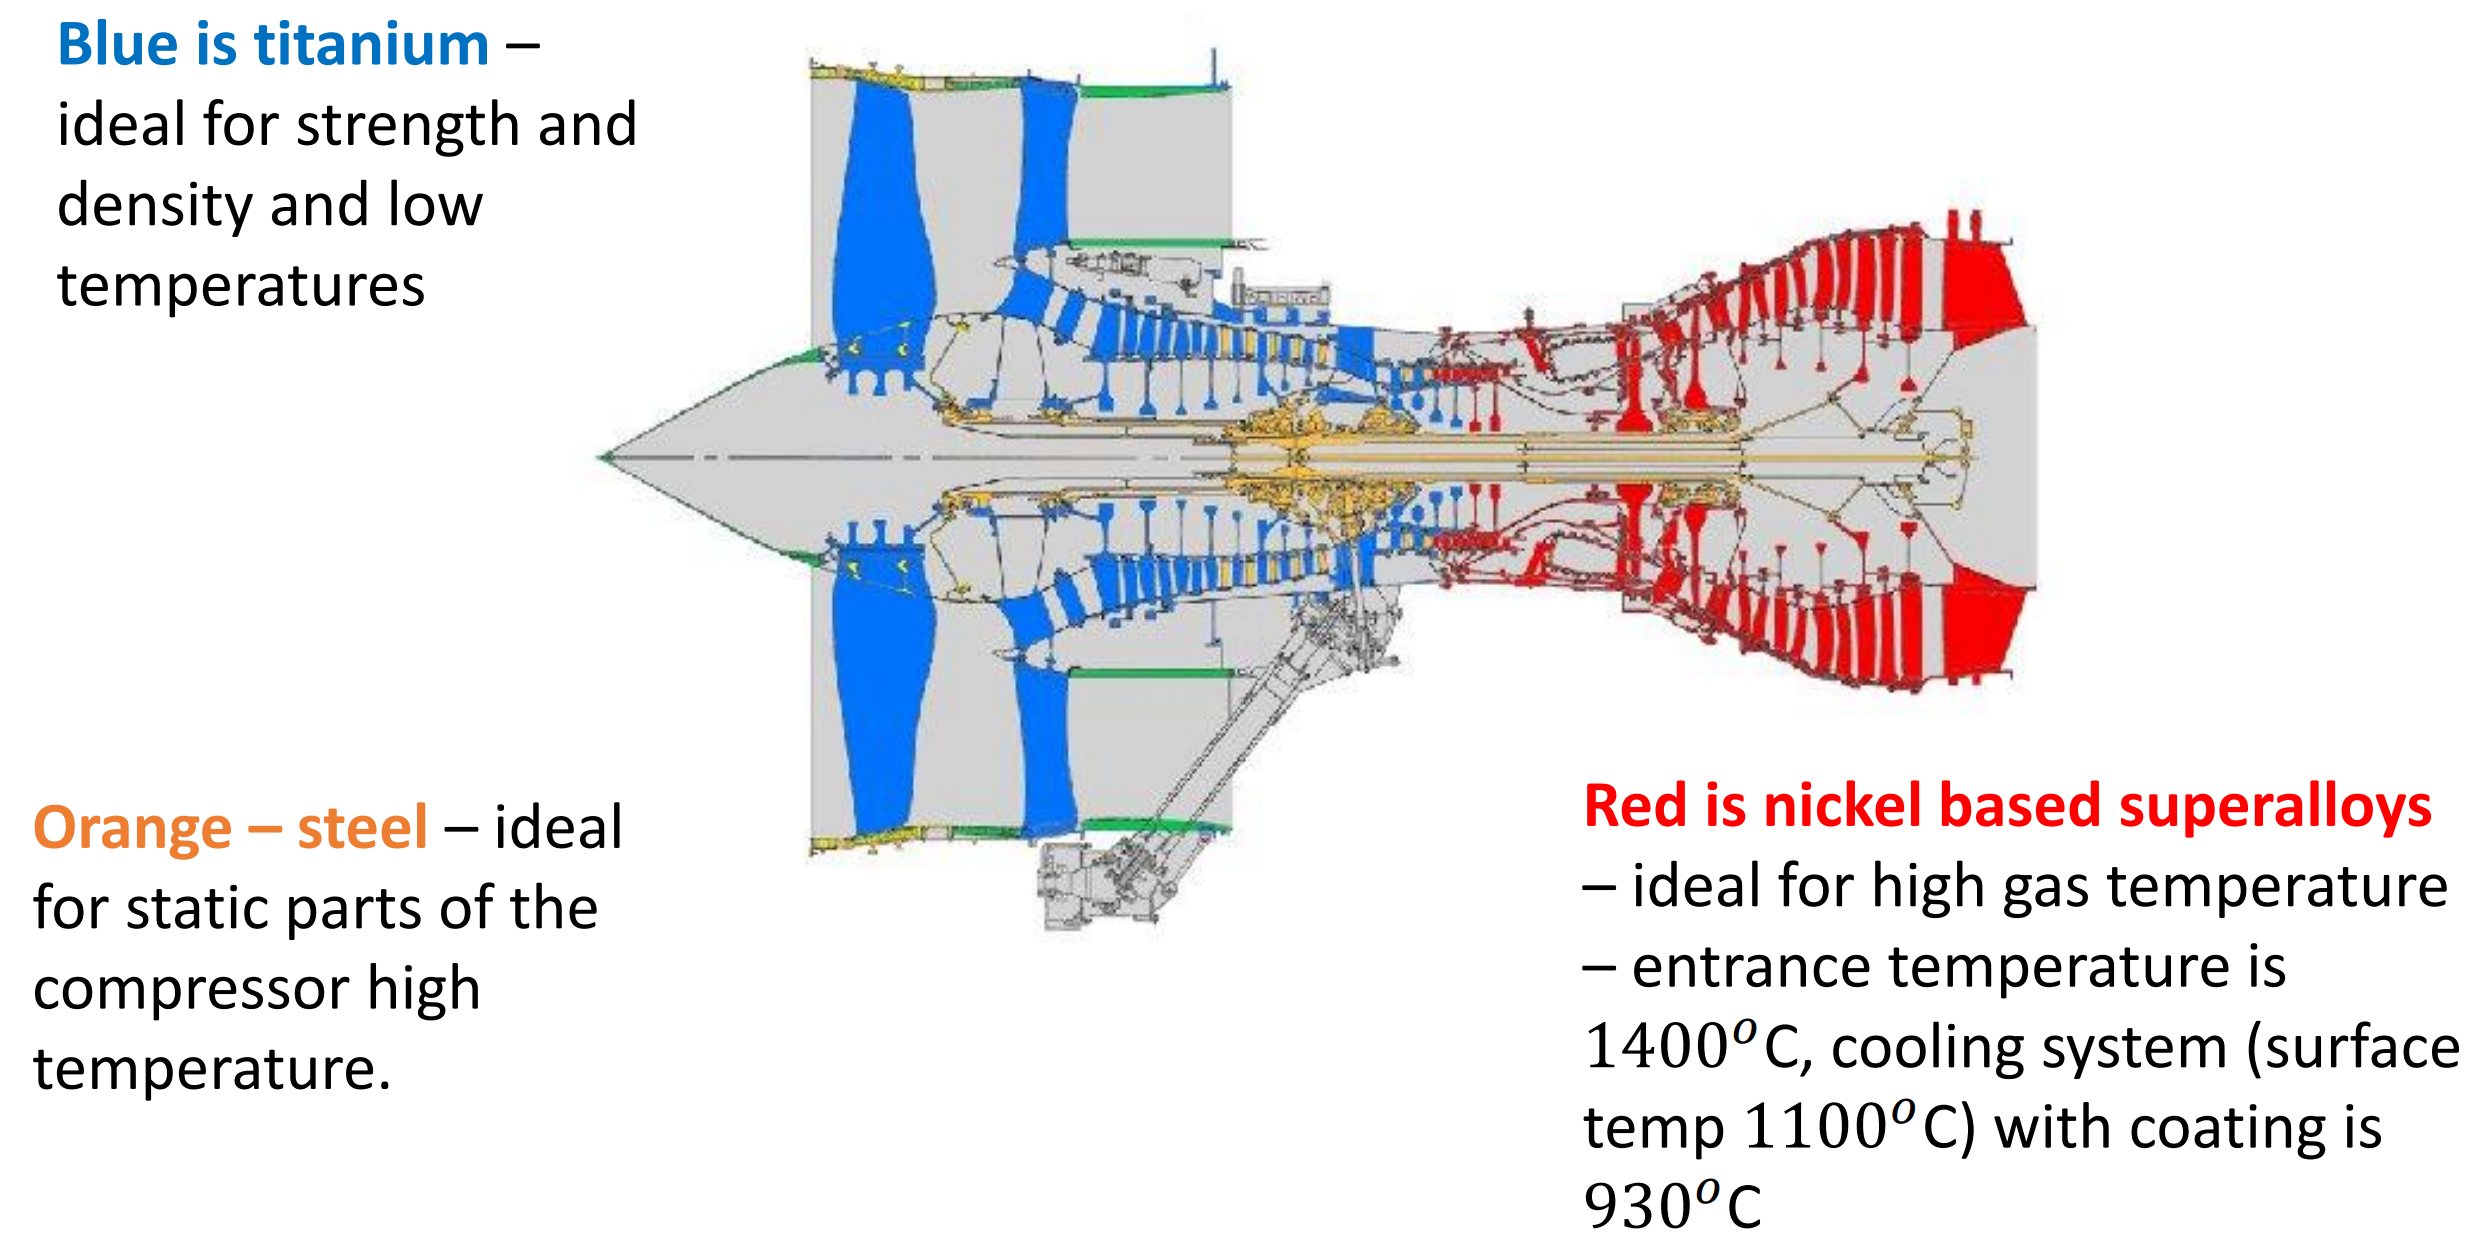
\includegraphics[width =\textwidth]{img/figure23.png}
    \caption{Usage of different alloys within the engine.}
\end{figure}
\begin{figure}[H]
    \centering
    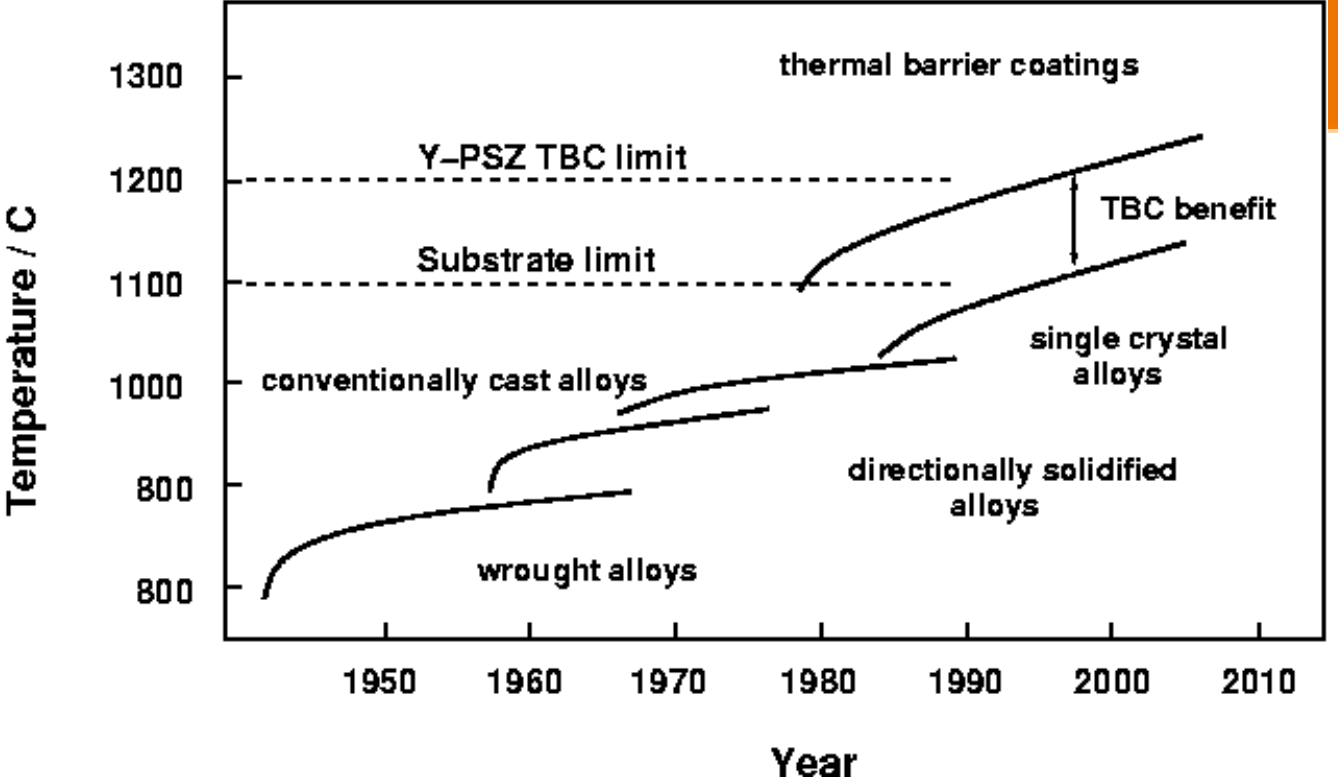
\includegraphics[width =0.8\textwidth]{img/figure24.png}
    \caption{Development of alloys.}
\end{figure}
Titanium - good for weight and strength (poor with heat).

Alloy improvement, directional and single-crystal solidifcation have contributed significantly, but arguably, the empahsis has been shifted to coating systems which have allowed an increase of gas temperatures up to \SI{1100}{\degree C}. Coatings in gas turbines serve a variety of purposes. A first requirement to operate turbines at higher temperatures was, of course, improved strength. Unfortunately, these conditions also mean severe oxidation / corrosion problems, and to make things worse, the improvement in mechanical properties of the base alloys was made at the expense of environmental resistance. 

The first purpose of coatings was to improve poor oxidation resistance of the base alloy (aluminide, Pt-aluminide, MCrAlY). A second type of coatings applied to high-temperature parts are known as thermal barrier coatings (TBC). These are ceramic coatings with very low thermal conductivity and thin (\SI{200}{\micro\meter}). Drop of 100-\SI{300}{\degree C} between the gas and metal surface temperatures but are `oxygen transparent' and do not prevent oxidation of the underlying substrate.
\subsection{Manufacturing process}
Aside from the alloy improvements, a major breakthrough was the development of directional solidification (DS) and single crystal (SC) production methods. These methods help greatly increase strength against fatigue and creep by aligning grain boundaries in one direction (DS) or by eliminating grain boundaries altogether (SC).

Recent generations of superalloys for single crystal turbine blades contain relatively high percentages of refractory elements such as Ta, W or Re which enhance the high-temperature mechanical properties. 

This is done at the expense of Cr and Al. Given the severe environmental conditions in which the blades operate, the removal of the elements (beneficical for oxidation resistance) implies even greater degradation problems. 

To reduce the oxidation corrosion resistance, an external coating is applied to the blades. Its purpose is to allow for the growth of a resistant oxide layer. Of all possible oxides $\alpha$-Al$_2$O$_3$ offers excellent protection and very low growth rates (in a minority of cases, Cr oxides are preferred). The composition of the coating must therefore be chosen carefulyl so as to ensure growth of $\alpha$-Al$_2$O$_3$.
\begin{figure}[H]
    \centering
    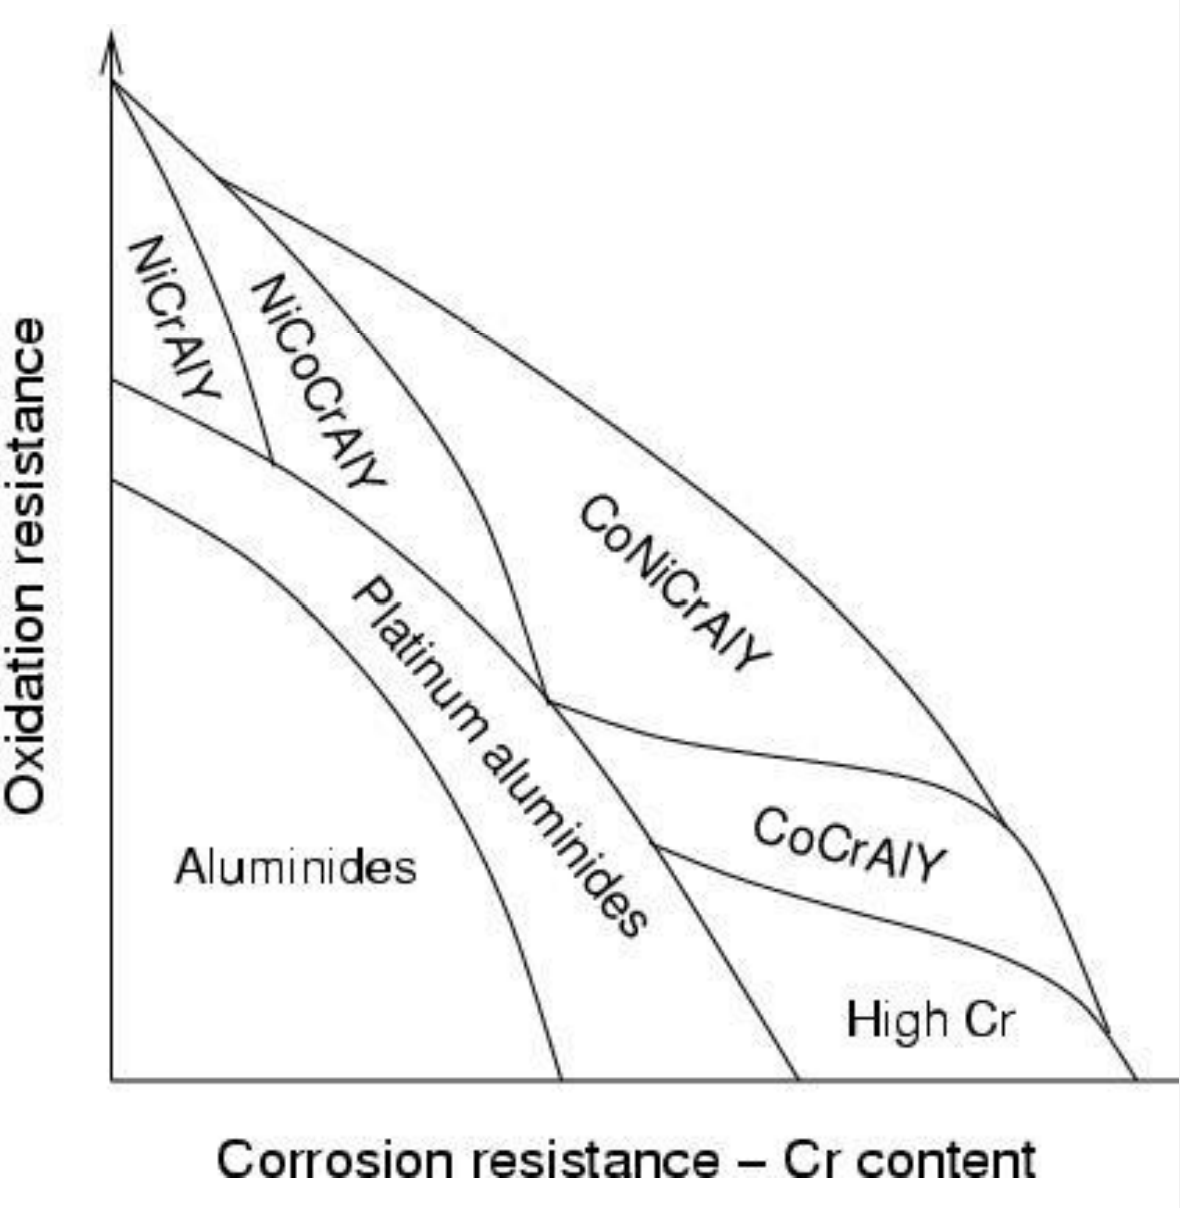
\includegraphics[width =0.6\textwidth]{img/figure25.png}
    \caption{Oxidation and corrosion resistance of different alloys.}
\end{figure}
\begin{figure}[H]
    \centering
    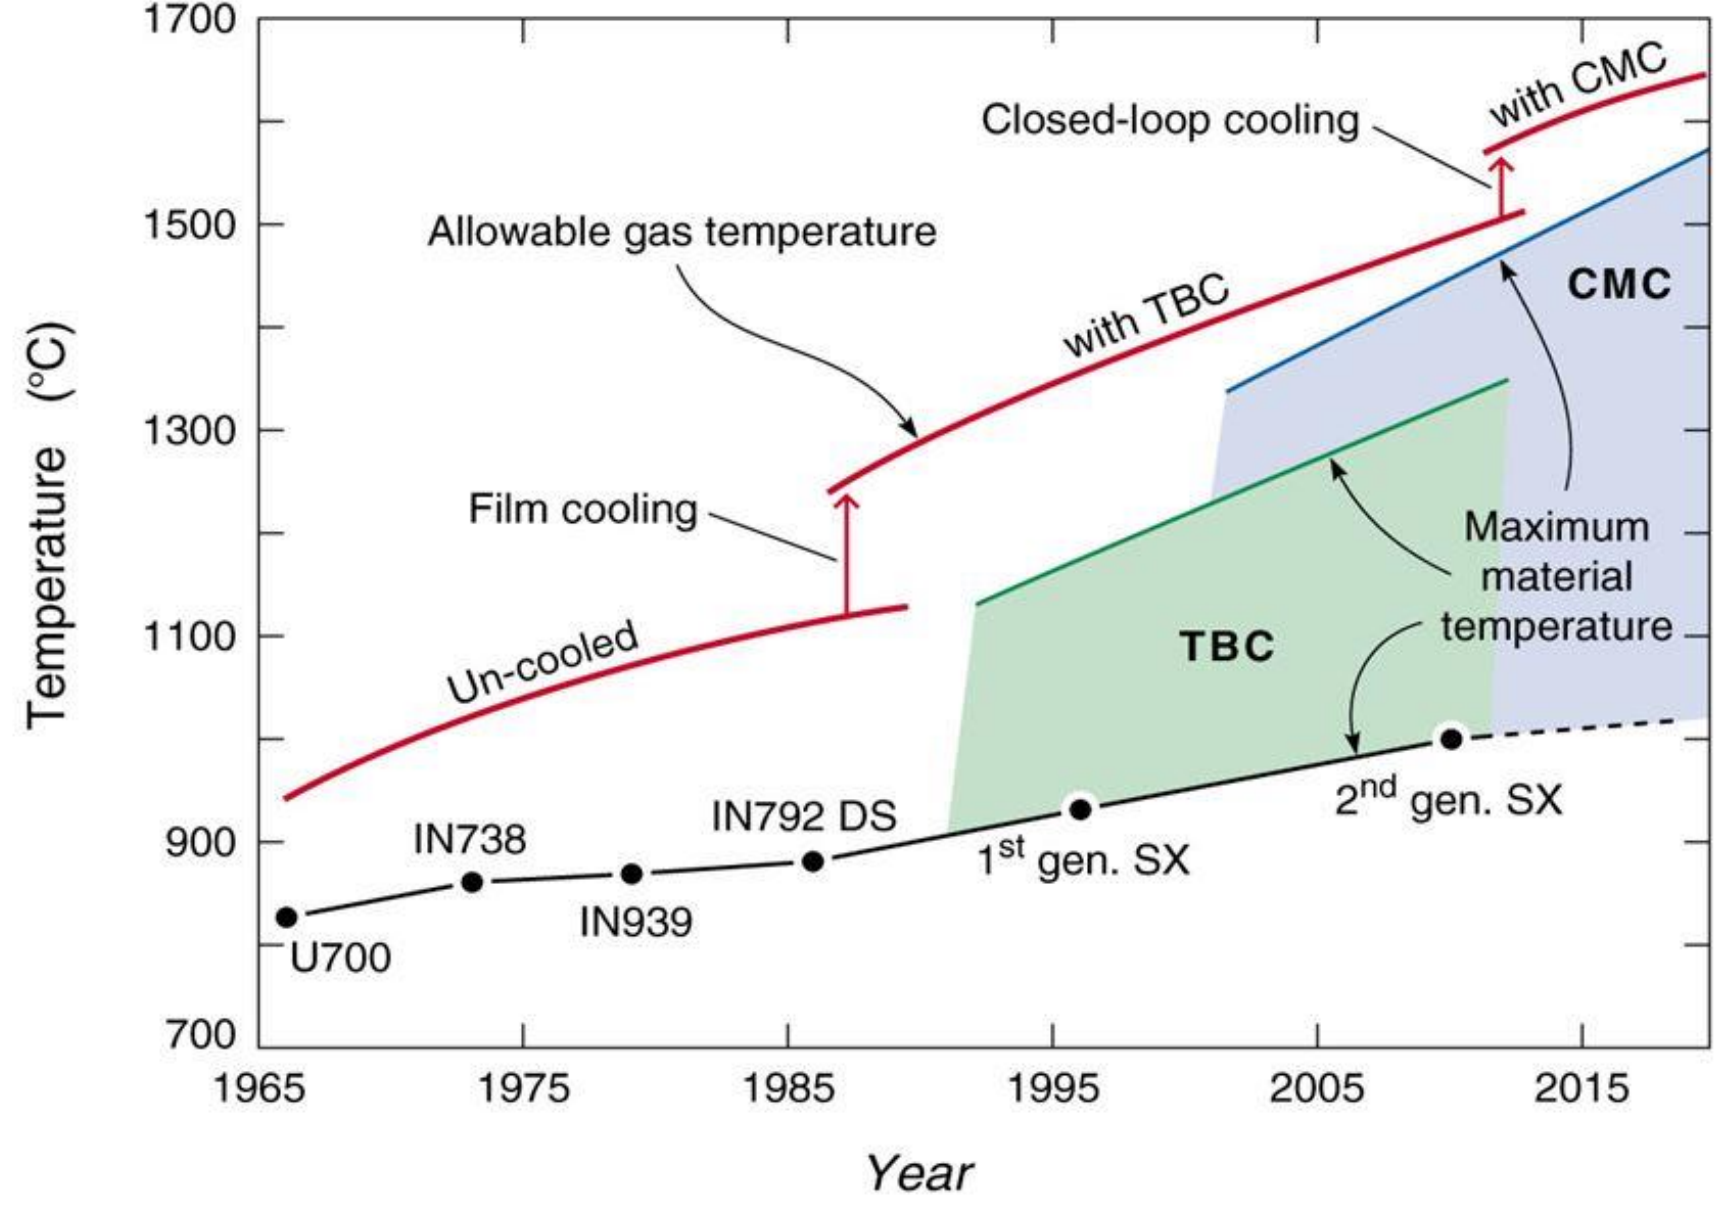
\includegraphics[width =0.8\textwidth]{img/figure26.png}
    \caption{Temperature resistance of TBCs and CMCs over the years.}
\end{figure}
TBC - thermal barrier coating. CMC - ceramic matrix composite.
\subsection{Thermal barrier coating}
Thermal barrier coatings (TBC) are advanced materials systems usually applied to metallic surfaces, such as on gas turbine or aero-engine parts, operating at elevated temperatures, as a form of exhaust heat management. These \SI{100}{\micro\meter} to \SI{2}{mm} coatings serve to insulate components from large and prolonged heat loads by utilising thermally insulating materials which can sustain an appreciable temperature difference between the load-bearing alloys and the coating surface.
\begin{figure}[H]
    \centering
    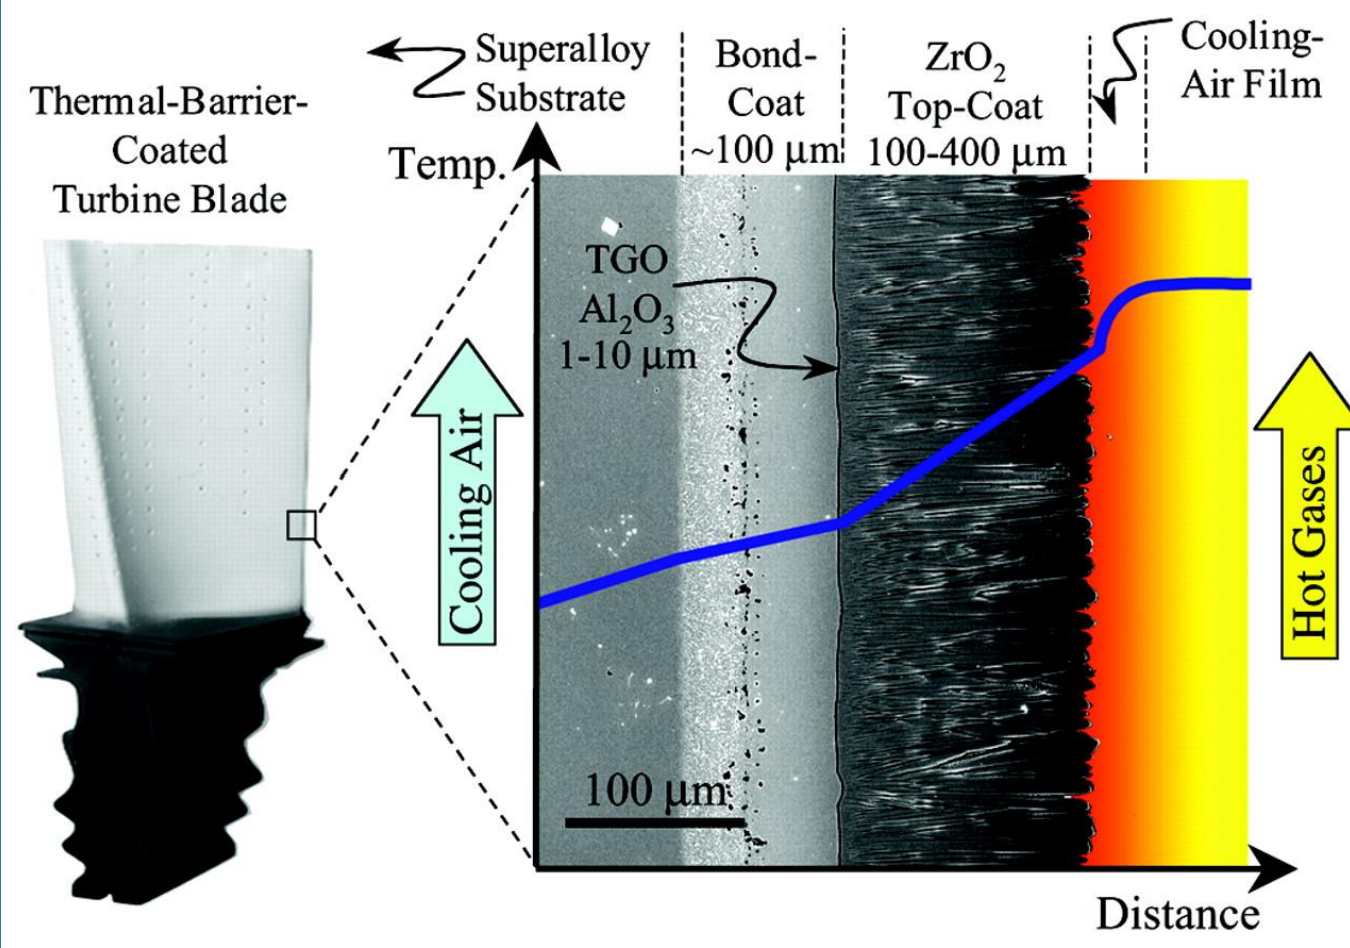
\includegraphics[width =0.6\textwidth]{img/figure27.png}
    \caption{Thermal barrier coatings (TBCs).}
\end{figure}
Four layers:
\begin{enumerate}
    \item The metal substrate
    \item Metallic bond coat
    \item Thermally-grown oxide (TGO)
    \item Ceramic topcoat. The ceramic topcoat is typically composed of yttria-stabilised zirconia (YSZ) which is desirable for having very low of conductivity while remaining stable at nominal operating temperatures typically seen in applications. This ceramic layer creates the largest thermal gradient of the TBC and keeps the lower layers at a lower temperature than the surface.
\end{enumerate}
\begin{figure}[H]
    \centering
    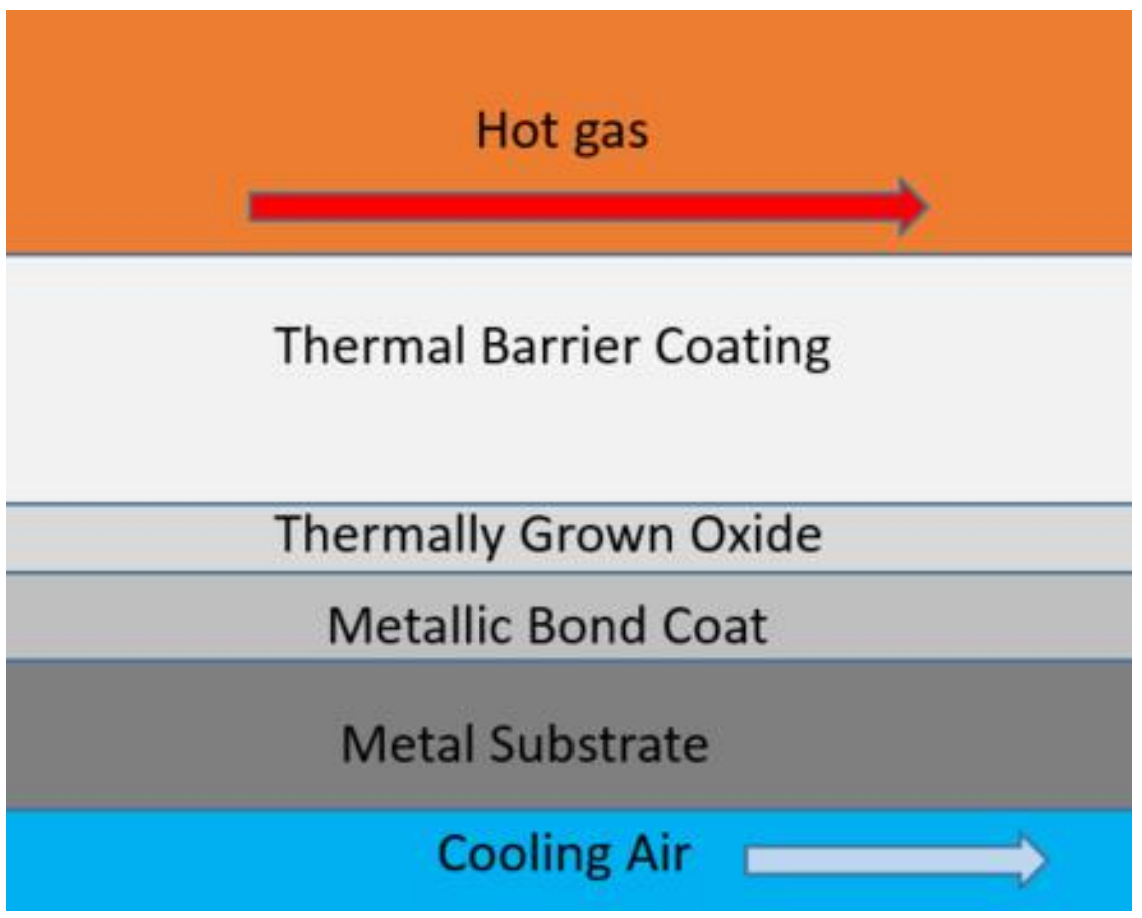
\includegraphics[width =0.6\textwidth]{img/figure28.png}
    \caption{Thermal barrier coating composition.}
\end{figure}
TBCs improved corrosion and oxidation resistance, both which became greater concerns as temperatures increased. First TBCs (1970s) were aluminide coatings. Ceramic coatings in 1980s which decreased turbine blade temperature by about \SI{90}{\degree C}, improve blade life, almost doubling the life of turbine blades in some cases.